\section{Experimental Causal Discovery}

%\subsection{Introduction}
\subsection{Types of Correlations}\label{sec:chocolote-Nobel-prize}

\begin{figure}[ht]
    \centering
%
\includegraphics[scale=0.4]{choco-nobel}

\includegraphics[width=0.8\textwidth]{messerli.pdf}
  \caption[Chocolate consumption and Nobel prizes]{Statisically significant correlation between chocolate consumption and Nobel prizes (correlation coefficient $R=0.69$, $p$-value for zero correlation $p=0.0004$.\protect\footnotemark}
\label{fig:choco-nobel}
\end{figure}

%\footnotetext{F.H. Messerli. \emph{Chocolate Consumption, Cognitive Function, and Nobel Laureates}. N Engl J. Med 2012; 367:1562-1564; DOI:10.1056/NEJMon1211064.} 
\footnotetext{This figure is inspired by \cite[Figure 1]{Mes12}. We made a similar visualization, but using newer data from \url{https://www.theobroma-cacao.de/wissen/wirtschaft/international/konsum} on chocolate consumption in 2017, and from \url{https://en.wikipedia.org/wiki/List_of_countries_by_Nobel_laureates_per_capita} on scientific Nobel laureates until 2019.}


\begin{Expl}\label{explanation:nobel_chocolate}
    What conclusions can we draw from this? Where does the correlation come from? Would the correlation hold under different conditions/circumstances?
    There are several explanations/stories that one could build around the observed correlation between the number of Nobel prizes $N$ and the chocolate consumption per capita $C$:
    \begin{enumerate}[label=\alph*)]
        \item $N$ causes $C$: ``Nobel prize winning countries like to celebrate with chocolate consumption.''
        \item $N$ is an effect of $C$: ``Chocolate contains brain enhancing chemicals.''
        \item Feedback between $N$ and $C$: Both stories hold.
        \item Selection bias between $N$ and $C$: ``$N$ and $C$ are actually independent, but the data used was biased. For example, only countries that end up close to the diagonal line in Figure~\ref{fig:choco-nobel} were included in the plot.''
        \item Functional constraints between $N$ and $C$: ``International regulations make sure that Nobel prizes and chocolate imports are subtracted/added if they violate a linear relationship.''
        \item $N$ and $C$ have a common cause: ``The wealth of a country determines both, how much money goes to science and also how much people can spend on chocolate.''
        \item Other explanations, e.g.\ measurement error, statistical coincidence, other forms of spurious correlations, combinations of all of these, etc.?
    \end{enumerate}
\end{Expl}



\begin{figure}[ht]
    \begin{subfigure}[b]{.32\textwidth}
    \centering
    \begin{tikzpicture}[scale=1, transform shape]
        \tikzstyle{every node} = [draw,shape=circle,color=blue]
        \node (N) at (0,0) {$N$};
        \node (C) at (3,0) {$C$};
        \draw[-{Latex[length=3mm, width=2mm]}, color=blue] (N) to (C);
    \end{tikzpicture}
    \subcaption{}
    \label{subfig:N-causes-C}
    \end{subfigure}
    \begin{subfigure}[b]{.32\textwidth}
    \centering
    \begin{tikzpicture}[scale=1, transform shape]
        \tikzstyle{every node} = [draw,shape=circle,color=blue]
        \node (N) at (0,0) {$N$};
        \node (C) at (3,0) {$C$};
        \draw[-{Latex[length=3mm, width=2mm]}, color=blue] (C) to (N);
    \end{tikzpicture}
    \subcaption{}
    \label{subfig:N-effect-C}
    \end{subfigure}
    \begin{subfigure}[b]{.32\textwidth}
    \centering
    \begin{tikzpicture}[scale=1, transform shape]
        \tikzstyle{every node} = [draw,shape=circle,color=blue]
        \node (N) at (0,0) {$N$};
        \node (C) at (3,0) {$C$};
        \draw[-{Latex[length=3mm, width=2mm]}, color=blue, bend left] (N) to (C);
        \draw[-{Latex[length=3mm, width=2mm]}, color=blue, bend left] (C) to (N);
    \end{tikzpicture}
    \subcaption{}
    \label{subfig:N-feedback-C}
    \end{subfigure}

    \medskip
    \begin{subfigure}[b]{.32\textwidth}
    \centering
    \begin{tikzpicture}[scale=1, transform shape]
        \tikzstyle{every node} = [draw,shape=circle,color=blue]
        \node (N) at (0,0) {$N$};
        \node (C) at (3,0) {$C$};
        \tikzstyle{every node} = [draw,shape=circle,color=black, fill=green]
        \node (S) at (1.5,-2) {$S$};
     %   \draw[-{Latex[length=3mm, width=2mm]}, color=blue] (N) to (C);
        \draw[-{Latex[length=3mm, width=2mm]}, color=green] (N) to (S);
        \draw[-{Latex[length=3mm, width=2mm]}, color=green] (C) to (S);
    \end{tikzpicture}
    \subcaption{}
    \label{subfig:N-selection-bias-C}
    \end{subfigure}
    \begin{subfigure}[b]{.32\textwidth}
    \centering
    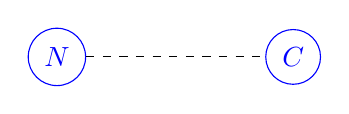
\begin{tikzpicture}[scale=1, transform shape]
        \tikzstyle{every node} = [draw,shape=circle,color=blue]
        \node (N) at (0,0) {$N$};
        \node (C) at (3,0) {$C$};
        \draw[-, dashed, color=black] (N) to (C);
    \end{tikzpicture}
    \subcaption{}
    \label{subfig:N-constrained-C}
    \end{subfigure}
    \begin{subfigure}[b]{.32\textwidth}
    \centering
    \begin{tikzpicture}[scale=1, transform shape]
        \tikzstyle{every node} = [draw,shape=circle,color=blue]
        \node (N) at (0,0) {$N$};
        \node (C) at (3,0) {$C$};
        \tikzstyle{every node} = [draw,shape=circle,color=red]
        \node (W) at (1.5,2) {$W$};
      %  \draw[-{Latex[length=3mm, width=2mm]}, color=blue] (N) to (C);
        \draw[-{Latex[length=3mm, width=2mm]}, color=red] (W) to (N);
        \draw[-{Latex[length=3mm, width=2mm]}, color=red] (W) to (C);
    \end{tikzpicture}
    \subcaption{}
    \label{subfig:N-common-cause-C}
    \end{subfigure}
    \caption{Graphical representations of different correlation inducing scenarios.}
    \label{fig:choco-nobel-graph}
\end{figure}


\begin{Disc}
    Correlation does not imply causation because there are other possible correlation inducing scenarios.
    Also, correlation is symmetric, causation is asymmetric.
\end{Disc}

%\begin{Exc}
%    Go through the news articles that claim statements like "drinking wine every day improves your health", etc., and look up the study and 
%\end{Exc}





\subsection{Causal Effects in the Real World}

\begin{Eg}[Does the thermometer cause the sun to rise?]
    \label{therm-sun}
    Consider an old type of thermometer ($T$) with a needle that can---for simplicity of arguments---either point to higher temperatures (up) or to lower temperatures (down).
    We also consider the state of the sun ($S$), which can either be up ($u$) or down ($d$).
    We then observe that $T$ correlates with $S$. For simplicity, we assume a one-to-one relationship:
    \[\begin{array}{c|c} 
        T & S \\ 
        \hline
        u & u \\
        d & d
    \end{array}\]
    The conditional distribution $P(S|T)$ then looks like this:
    \begin{align*}
        P(S=u|T=u) & = 1, \\
        P(S=u|T=d) & = 0, \\
        P(S=d|T=u) & = 0, \\
        P(S=d|T=d) & = 1.
    \end{align*}
    If we are cold we are now tempted to try changing the needle in the thermometer in order to make the sun rise and warm us up.\\
What is wrong with our analysis?
\end{Eg}

\begin{Disc}
    The example \ref{therm-sun} makes clear that there is a difference between:
    \begin{enumerate}
        \item \emph{Observing} the positions of the thermometer needle $T$ and the sun $S$, resulting in an \emph{observational} data set, 
            leading to an estimate of $P(S|T)$.
        \item \emph{Interacting} with the thermometer needle $T$ and getting the sun's response $S$, resulting in an \emph{interventional} data set, leading to estimates for $P(S|\doit(T))$:
                \begin{align*}
                    P(S=u|\doit(T=u)) & = 0.5, \\
                    P(S=u|\doit(T=d)) & = 0.5, \\
                    P(S=d|\doit(T=u)) & = 0.5, \\
                    P(S=d|\doit(T=d)) & = 0.5.
    \end{align*}
    \end{enumerate}
\end{Disc}

\begin{Def}[Causal effect---informal definition]
    \label{def-causality-real}
    We say that a variable $X$ has a \emph{causal effect} on another variable $Y$ if
    \emph{forcing} $X$ to take on a value $x$, the distribution of $Y$ explicitly depends on $x$, that is:
%    \[ \exists x_0,x_1 \in \Xcal:\qquad P(Y|\doit(X=x_0)) \neq P(Y|\doit(X=x_1)). \]
%    \Joris{Update to:
    \[ \exists x \in \Xcal:\qquad P(Y|\doit(X=x)) \neq P(Y). \]
%    }
\end{Def}
\begin{defmark}
\begin{Rem}
    \begin{enumerate}
        \item 
    Again, note that example \ref{therm-sun} shows that the condition in definition \ref{def-causality-real} is different from:
%    \[ \exists x_0,x_1 \in \Xcal:\qquad P(Y|X=x_0) \neq P(Y|X=x_1), \]
    \[ \exists x \in \Xcal:\qquad P(Y|X=x) \neq P(Y). \]
    which just uses the conditional distributions instead of the interventional distributions.
        \item Also note, that the `$\doit$-operators' are not operators on the observational distribution $P(X,Y)$ or $P(Y|X)$, etc., or on the corresponding observational data sets. They reflect actions/interventions in the real world leading to different distributions and corresponding data sets. 
        \item There are usually many possible intervention values and targets one can think of, leading to many different interventional distributions and data sets.
        \item One may think of the observational distribution as a special case of an interventional distribution (where we intervene by doing nothing).
    \end{enumerate}
\end{Rem}
\end{defmark}

\subsection{Randomized Controlled Trials (RCT)} % - The gold standard for experimental causal discovery }

\begin{claimmark}
\begin{Prn}[Randomized Controlled Trial (RCT)]\label{prn:rct}
 Assume we want to know if `treatment' variable $X$ has a causal effect on `outcome' variable $Y$, i.e.\ we want to estimate the deviation between:
$ P(Y|\doit(X=x_0))$ and  $P(Y|\doit(X=x_1))$. For this we have test subjects $w_1,\dots,w_N$.
A \emph{Randomized Controlled Trial} then follows the following steps:
\begin{enumerate}
    \item Split the population of test subjects into 2 groups (`test group' $C_1$ vs.\ `control group' $C_0$) by random lot (or fair coin flips).
    \item Give every test subject $w_n \in C_1$ from `test group' the treatment $x_1$ and the ones  $w_n \in C_0$ from `control group' the control treatment $x_0$.
    \item Measure the outcome $y_n$ for each test subject $w_n$ and estimate the deviation: \[D:=d(P(Y|\doit(X=x_0)),P(Y|\doit(X=x_1))).\]
    \item Do a statistical test if the deviation $D$ is significantly different from $0$. 
    \item If it is significantly different from 0 we can conclude a \emph{causal effect} of $X$ on $Y$, otherwise not.
\end{enumerate}
\end{Prn}
\end{claimmark}

\begin{Rem}
  The notion of a randomized controlled trial goes back several centuries. It was already described in 1648 by Flemish physician Jan Baptista van Helmont \cite{vanHelmont1648}:
  ``Let us take from the itinerants' hospitals, from the camps or from elsewhere 200 or 500 poor people with fevers, pleurisy etc. and divide them in two: let us cast lots so that one half of them fall to me and the other half to you. I shall cure them without blood-letting or perceptible purging, you will do so according to your knowledge (nor do I even hold you to your boast of abstaining from phlebotomy or purging) and we shall see how many funerals each of us will have: the outcome of the contest shall be the reward of 300 florins deposited by each of us. Thus shall your business be concluded. O Magistrates to whose hearts the health of your people is dear; let the trial be made for the public good, in order to know the truth, for the sake of your life and soul and for the health of all the people, sons, widows and orphans. Let there be a real debate to find the means of cure.''
\end{Rem}

\begin{Eg}
    Example applications of randomized controlled trials are:
    \begin{enumerate}
        \item drug or vaccine testing,
        \item advertisement placement,
        \item evaluating public policies, etc.
        \item A. Banerjee, E. Duflo, M. Kremer got the Nobel Prize in Economics 2019 for using RCTs in poverty research, e.g.\: improving school attendance and performance in poor areas via giving different towns different incentives (e.g.\ text books vs. deworming medicine vs. control groups).
    \end{enumerate}
\end{Eg}

\begin{Disc}
    \begin{enumerate}
        \item An RCT is an `interventional study' (in contrast to just `observational study') since we control the treatment and `force' it onto the test subjects.
        \item Randomized Controlled Trials are considered the gold standard for experimental causal discovery.
        \item To further avoid biases one usually insists on double/triple blind RCT studies, 
            i.e.\ noone directly involved in the study knows who got which treatment 
            (e.g.\ neither the doctor, the experimenter, the patient, etc.). 
        \item Often RCTs cannot be done for ethical reasons (e.g.\ ``smoking causes cancer'' research).
        \item Sometimes RCTs require too many resources to be feasible.
    \end{enumerate}
\end{Disc}


\begin{Exc}
    Go online, find news like ``drinking wine every day is good for your health'' or ``chewing gum causes diabetes'', etc., 
    look up the original research paper and check:
    \begin{enumerate}
        \item if they did interventional studies (like RCT) or just observational studies,
        \item in case of an RCT, whether it was double/triple blind,
        \item otherwise, if (and how) they ruled out other correlation inducing scenarios,
        \item what bias could have possibly been introduced through the data collecting process,
        \item how big the data set was, what assumptions were made, what statistical methods were used, etc.,
        \item what other `stories' you could come up with in order to explain the data.
    \end{enumerate}
    Write down your findings and talk to others about it.
\end{Exc}
